\section{Where and how much: a map of the damage}
\label{sec:map}

\subsection{One Gaussian mode: exact formulas}
Consider a Gaussian mode of position standard deviation $s$ and measure lengths in units of $s$.
The result depends only on $r/\kappa$, $\smin/s$, $\smax/s$, the initial velocity scale and $M$; the time scale $\beta$ drops out at fixed $r/\kappa$.
Write the clipped output covariance as $\Sigma=C+E$, with $C$ the true covariance.
Formulas use the log ratio $L=\log(\Sigma_{xx}/C_{xx})$; percentages quote the relative change of the variance, $e^{L}-1$, and the two agree for small $|L|$.

\begin{derived}[error equation]
\label{der:error}
In reverse time $\tau=T-t$,
\begin{equation}
\begin{aligned}
&\frac{dE}{d\tau}=AE+EA^{\top}-\Gm,\quad E(0)=0,\\
&A=-B-\Gp C^{-1} .
\end{aligned}
\label{eq:error}
\end{equation}
With $\Gm=2(\kappa-r)\sigma^2uu^{\top}$, the shrinkage is
\begin{equation}
\begin{aligned}
&L=\log\Bigl(1-(\kappa-r)\,\frac{K_{xx}(r)}{C_{xx}(0)}\Bigr),\\
&K=\int_0^T 2\sigma^2\,\Phi\,uu^{\top}\Phi^{\top}dt\succeq0 ,
\end{aligned}
\label{eq:exactform}
\end{equation}
Here $\tau=0$ is the start of sampling ($\sigma=\smax$), and $E(0)=0$ because the prior is exact. $A$ depends on time through $\Gp$ and $C$. $\Phi$ is the propagator of the homogeneous part of Eq.~\eqref{eq:error}, $d\Phi/d\tau=A\Phi$, from forward time $t$ to the end of sampling at $t=0$, and $C_{xx}(0)$ is the target variance, the data blurred by $\smin$.
\end{derived}

Equation~\eqref{eq:error} follows by subtracting the moment equation of the true covariance from that of sampler~\Sa{}.
Equation~\eqref{eq:exactform} agrees with the full moment equations to a relative $10^{-11}$.
The shrinkage is thus $(\kappa-r)$ times a non-negative quantity; three limits follow.

\begin{derived}[limits]
\label{der:limits}
(a) \emph{Threshold slope}: $L\simeq-(1-r/\kappa)\,\kappa K_{xx}(\kappa)/C_{xx}(0)$.
The slope is $0.035$ for the setup of Sec.~\ref{sec:exact}, and agrees with the full solution at $r/\kappa=0.99$ to within 0.3--1.1\%.
(b) \emph{Noise-dominated limit} ($\smin\gg s$): $E=\sigma^2F$, with $F$ the solution of the constant Lyapunov equation $(A+rI)F+F(A+rI)^{\top}=2(\kappa-r)uu^{\top}$.
The limit $L_\infty=\log(1+F_{xx})$ depends only on $r/\kappa$ and $M$.
For $M=1/4$ the variance changes by $e^{L_\infty}-1=F_{xx}=-21.6\%$, $-13.8\%$ and $-3.2\%$ at $r/\kappa=0.1, 0.5, 0.9$.
(c) \emph{$r\to0$ at fixed $\smin$}: freezing $\sigma=\smin$ gives $-2.9\%$ for the setup of Sec.~\ref{sec:exact}.
This is not a bound for large $M$, where the shrinkage is not monotone in $r$.
\end{derived}

\begin{observation}[the damage is made at the end]
\label{obs:local}
$E$ is linear in its source, so the shrinkage can be split by the band of $\sigma$ in which $\Gm$ acts.
In every setting examined, essentially all of the final shrinkage is injected between $\smin$ and about $2\smin$ [Fig.~\ref{fig:map}(c)].
Errors injected at larger $\sigma$ relax before the end.
Accordingly, $\smax$ has no effect: $L$ is unchanged, to a relative $10^{-11}$, from $\smax=5s$ to $5000s$.
\end{observation}

\begin{observation}[map]
\label{obs:map}
With the CLD mass $M=1/4$ and $\smin\ll s$, the variance shrinks by $2.6\%$ ($\smin=s/16$) to $4.6\%$ ($\smin=s/100$) even at $r/\kappa=0.1$, and never by $10\%$ [Fig.~\ref{fig:map}(a)].
It exceeds $10\%$ when $\smin\gtrsim s$ (for small $r/\kappa$) or when $M$ is far from $1/4$ ($M\lesssim0.03$, or $M\gtrsim3$ with $\smin=s/2$) [Fig.~\ref{fig:map}(b)], reaching about $25\%$.
Neither the initial velocity scale nor $\smax$ brings it to $10\%$.
\end{observation}

\begin{figure*}[t]
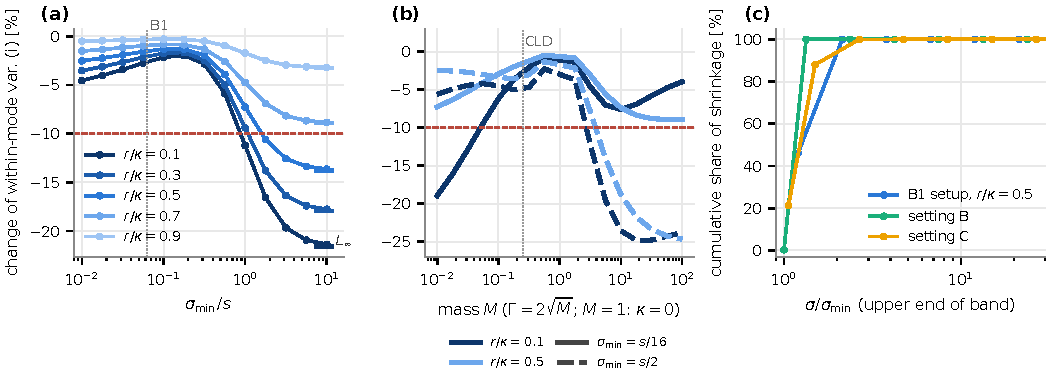
\includegraphics[width=\textwidth]{figures/fig2_map}
\caption{Map of the damage (one Gaussian mode, exact moment equations).
(a) Change of the within-mode variance of \Sa{} against $\smin/s$ for the CLD mass; the bars at the right are the noise-dominated limits, plotted as $e^{L_\infty}-1$ (Derived result~\ref{der:limits}b).
(b) Against the mass $M$ ($\Gamma=2\sqrt M$, $\kappa$ fixed by $\beta$), at $r/\kappa=0.1$ (dark) and $0.5$ (light), for $\smin=s/16$ (solid) and $s/2$ (dashed).
The red dashed line marks $-10\%$.
(c) Cumulative share of the final shrinkage injected below a given $\sigma$: the damage is made between $\smin$ and about $2\smin$.}
\label{fig:map}
\end{figure*}

\subsection{Eight modes}
We chose three settings from the map and checked them with the eight-mode mixture, using the method of Sec.~\ref{sec:exact}; $\beta$ is set so that $\kappa=2$ in each.

\begin{observation}[mixtures]
\label{obs:mixture}
In all three settings of Table~\ref{tab:mixture} the clipped sampler shrinks the within-mode variance by more than $10\%$, and \Sb{} and \Sc{} stay correct ($|100L|\leq0.3$).
The shift towards the mode centres is visible in the distribution of distances from the centre.
\end{observation}

\begin{table}[t]
\caption{Eight-mode mixtures, exact score, five seeds, step-extrapolated: change of the within-mode position variance of \Sa{}, paired with \Sb{}, and the one-mode theory. Setting B uses the CLD mass.}
\label{tab:mixture}
\begin{ruledtabular}
\begin{tabular}{lcccc}
 & $M$ & $\smin$ & $r/\kappa$ & mixture (theory) \\
\hline
A & $0.01$ & $s/16$ & $0.2$ & $-15.1\%$ ($-15.4\%$) \\
B & $1/4$ & $1.78\,s$ & $0.3$ & $-11.1\%$ ($-13.8\%$) \\
C & $10$ & $s/2$ & $0.5$ & $-18.6\%$ ($-18.8\%$) \\
\end{tabular}
\end{ruledtabular}
\end{table}

Setting B keeps the CLD flow unchanged and leaves a final blur comparable to the mode width; setting C changes the mass.
One observation remains open: in setting A the velocity variance shrinks by $-16.7\%$ in the mixture, against $-6.0\%$ for one mode, while the positions agree with the theory.
A single-mode control reproduces the theory, so this is a genuine mixture effect, and it is not explained here.
